\section{Newton's Method}

\textbf{Find zeros}: $x_{t+1} = x_t - \frac{f(x_t)}{f^\prime(x_t)}$. This is to solve the first-order approximation: $f(x_t)+f^\prime(x_t)(x-x_t) = 0$.

\textbf{Find minimum}: $x_{t+1} = x_t - \frac{f^\prime(x_t)}{f^{\prime\prime}(x_t)}$. This is to search zeros of $f^\prime$. Generally, $x_{t+1} = x_t - \nabla^2 f(x_t)^{-1} \nabla f(x_t)$. (10.3) $x_{t+1} = \argmin f(x_t) + \nabla f(x_t)^\top (x-x_t) + \frac{1}{2}(x-x_t)^\top \nabla^2 f(x_t) (x-x_t)$.

\textbf{Analysis}:
\begin{enumerate}
    \item \textbf{Nondegenerate quadratic function}: (10.1) for $f(x) = \frac{1}{2}x^\top M x - q^\top x +c$ with invertible symmetric $M$, Newton's method yields $x_1 = x^* = M^{-1} q$ for any $x_0$.
    \item \textbf{Affine invariance}: (10.2) let $f$ be twice differentiable, $A$ invertible and $g(y)=Ay+b$. Define $N_h(x) = x - \nabla^2 h(x)^{-1}\nabla h(x)$, then $N_{f\circ g}=g^{-1} \circ N_f \circ g$.
    \begin{center}
        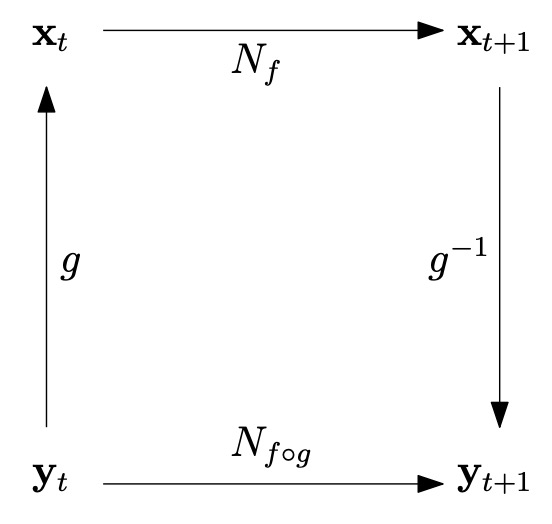
\includegraphics[width=.4\linewidth]{imgs/newton-affine.jpg}
    \end{center}
    \item \textbf{Bounded inverse Hessian and Lipschitz continuous Hessian}: (10.4) assume $f$ is twice continuously differentiable, $\|\nabla^2 f(x)^{-1}\| \le 1/\mu$ and $\|\nabla^{2} f(x) - \nabla^2 f(y)\| \le B\|x-y\|$ for any $x, y \in X$. Then we have $\|x_{t+1}-x^*\| \le \frac{B}{2\mu}\|x_t - x^*\|^2$ if a critical point $x^*$ exists in $X$. Proof: Define $H(x)=\nabla^2 f(x)$. $x_{t+1}-x^* = x_t - x^* + H(x_t)^{-1}(\nabla f(x^*) - \nabla f(x_t)) = x_t - x^* + H(x_t)^{-1} \int_0^1 H(x_t+u(x^*-x_t))(x^* - x_t) du = H(x_t)^{-1} \int_0^1 (H(x_t + u(x^* - x_t)) - H(x_t))(x^* - x_t) du$. Therefore, we have $\|x_{t+1}-x^*\| \le \|H(x_t)^{-1}\| \|x^* - x_t\| \int_0^1 \|H(x_t + u(x^* - x_t)) - H(x_t)\| du \le \frac{1}{\mu} \|x_t - x^*\|^2 B \int_0^1 u du = \frac{B}{2\mu} \|x_t-x^*\|^2$.
    \item \textbf{Fast convergence if near}: (10.5) under the assumption of (10.4), if $\|x_0-x^*\| \le \mu/B$, then $\|x_T - x^*\| \le \frac{\mu}{B}(\frac{1}{2})^{2^T-1}$. Proof: induction on (10.4).
    \item \textbf{Global convergence for strongly convex and smooth functions}: with $\gamma=\mu/L$, (scaled) Newton's method $x_{t+1}=x_t - \gamma \nabla^2 f(x_t)^{-1} \nabla f(x_t)$ satisfies $f(x_t) - f^* \le (1-\frac{\mu^2}{L^2})^t (f(x_0) - f^*)$. Note that the constant is worse than GD. Proof: expand $f(x_{t+1}) - f(x_t)$ by smoothness, then use $\frac{1}{L}\le \|H_t^{-1}\| \le \frac{1}{\mu}$ and $\|\nabla f(x_t)\|^2 \ge 2\mu (f(x_t)-f^*)$.
\end{enumerate}